 % The main file for CAMP reports
 % Don't put any content in here. 
 % Don't even include content files by using \input or \inlcude. 
 % Put your content to TEXT.TEX or include it there using \input.
 % Uses:
 %		SETTINGS.TEX	contains the settings for this document
 %		COMMANDS.TEX	contains commands which can be used while writing
 %		INFO.TEX			contains the author, title and so on for the cover
 %		COVER.TEX			formats the front cover of the document
 %		ABSTRACT.TEX	contains the abstract to be included (if needed)
 %		TEXT.TEX			contains the actual content of the document
 %		BIB.BIB				containt the BibTeX entries for the document
 
 
%% Draft document mode
%% Final document
\documentclass[11pt,a4paper,bibtotoc,idxtotoc,headsepline,footsepline,footexclude,BCOR12mm,DIV13]{scrbook}

%\documentclass[11pt,a4paper,bibtotoc,idxtotoc,headsepline,footsepline,footexclude,BCOR20mm,DIV10]{scrbook}

% KOMA-Optionen:
%  bibtotoc: include bibliography in table of contents
%  idxtotoc: include index in table of contents
%  headsepline: use horizontalline under heading
%  BCOR: binding correcion (Bindungskorrektur) (e.g.: BCOR5mm)
%  DIV: Number of sheet sections (used for layout) (e.g.: DIV12) 



% include title and author information for the cover
% Set here the title, authors and other stuff to be used for the cover
% This file is used by MAIN.TEX

% set title, authors and stuff for the cover
\def\doctype{Diplomarbeit in Informatik}
\def\title{Semi-automated detection of sanitization, autehntication and declassification errors in UML state charts}
\def\titleGer{Halbautomatische Erkennung von Sanitisierungs-, Authenifizierungs- und Deklassifierungsfehlern in UM L-Zusantsdiagrammen}
\def\author{Md Adnan Hossain Rabbi}
\def\date{November 15, 2015}

% text to appear in the footer
\def\footertext{}

% include settings
% Included by MAIN.TEX
% Defines the settings for the CAMP report document

\renewcommand{\sectfont}{\normalfont \bfseries}        % Schriftart der Kopfzeile

% manipulate footer
\usepackage{scrpage2}
\pagestyle{scrheadings}
\ifoot[\footertext]{\footertext} % \footertext set in INFO.TEX
%\setkomafont{pagehead}{\normalfont\rmfamily}
\setkomafont{pagenumber}{\normalfont\rmfamily}

%% allow sophisticated control structures
\usepackage{ifthen}

% use Palatino as default font
\usepackage{palatino}

% enable special PostScript fonts
\usepackage{pifont}

% make thumbnails
\usepackage{thumbpdf}

%to use the subfigures
\usepackage{subfigure}


\usepackage{colortbl}


%% show program code\ldots
%\usepackage{verbatim}
%\usepackage{program}

%% enable TUM symbols on title page
\usepackage{styles/tumlogo}
\usepackage{url}

\usepackage{multirow}

%% use colors
\usepackage{color}

%% make fancy math
\usepackage{amsmath}
\usepackage{amsfonts}
\usepackage{amssymb}
\usepackage{textcomp}
\usepackage{yhmath} % f�r die adots 
%% mark text as preliminary
%\usepackage[draft,german,scrtime]{prelim2e}

%% create an index
\usepackage{makeidx}

% for the program environment
\usepackage{float}

%% load german babel package for german abstract
%\usepackage[german,american]{babel}
\usepackage[german,english]{babel}
\selectlanguage{english}

% use german characters as well
\usepackage[latin1]{inputenc}       % allow Latin1 characters

% use initals dropped caps - doesn't work with PDF
%\usepackage{dropping}


\usepackage{styles/shortoverview}
%----------------------------------------------------
%      Graphics and Hyperlinks
%----------------------------------------------------

%% check for pdfTeX
\ifx\pdftexversion\undefined
 %% use PostScript graphics
 \usepackage[dvips]{graphicx}
 \DeclareGraphicsExtensions{.eps,.epsi}
 \graphicspath{{figures/}{figures/review}} 
 %% allow rotations
 \usepackage{rotating}
 %% mark pages as draft copies
 %\usepackage[english,all,light]{draftcopy}
 %% use hypertex version of hyperref
 \usepackage[hypertex,hyperindex=false,colorlinks=false]{hyperref}
\else %% reduce output size \pdfcompresslevel=9
 %% declare pdfinfo
 %\pdfinfo { 
 %  /Title (my title) 
 %  /Creator (pdfLaTeX) 
 %  /Author (my name) 
 %  /Subject (my subject	) 
 %  /Keywords (my keywords)
 %}
 %% use pdf or jpg graphics
 \usepackage[pdftex]{graphicx}
 \DeclareGraphicsExtensions{.jpg,.JPG,.png,.pdf,.eps}
 \graphicspath{{figures/}} 
 
 %% Load float package, for enabling floating extensions
 \usepackage{float}
 
 %% allow rotations
 \usepackage{rotating}
 %% use pdftex version of hyperref
 \usepackage[pdftex,colorlinks=true,linkcolor=red,citecolor=red,%
 anchorcolor=red,urlcolor=red,bookmarks=true,%
 bookmarksopen=true,bookmarksopenlevel=0,plainpages=false%
 bookmarksnumbered=true,hyperindex=false,pdfstartview=%
 ]{hyperref}
%
%\usepackage[pdftex,colorlinks=false,linkcolor=red,citecolor=red,%
% anchorcolor=red,urlcolor=red,bookmarks=true,%
% bookmarksopen=true,bookmarksopenlevel=0,plainpages=false%
% bookmarksnumbered=true,hyperindex=false,pdfstartview=%
% ]{hyperref}
\fi




%% Fancy chapters
%\usepackage[Lenny]{fncychap}
%\usepackage[Glenn]{fncychap}
%\usepackage[Bjarne]{fncychap}

%\usepackage[avantgarde]{quotchap}

% set the bibliography style
%\bibliographystyle{styles/bauermaNum}
%\bibliographystyle{alpha}
\bibliographystyle{plain}

% include commands
% Commands to be used within the TUM report document
% Included by MAIN.TEX
% Please include your own cool commands here. 
% Be only sure to comment it sufficiently so others can use it.

%-------------------------------------------------------------
%                      Own Commands
%-------------------------------------------------------------


%-------------------------------------------------------------
% math stuff -------------------------------------------------

% nice R, N, C
\newcommand{\nat}{\mathbb{N}}
\newcommand{\real}{\mathbb{R}}
\newcommand{\compl}{\mathbb{C}}



% norm
\newcommand{\norm}[1]{\left\| #1 \right\|}

% un demi
\newcommand{\half}{\frac{1}{2}}

% parantheses
\newcommand{\parenth}[1]{ \left( #1 \right) }
\newcommand{\bracket}[1]{ \left[ #1 \right] }
\newcommand{\accolade}[1]{ \left\{ #1 \right\} }
%\newcommand{\angle}[1]{ \left\langle  #1 \right\rangle }

% partial derivative: %#1 function, #2 which variable
% simple / single line version
\newcommand{\pardevS}[2]{ \delta_{#1} f(#2) }
% fraction version
\newcommand{\pardevF}[2]{ \frac{\partial #1}{\partial #2} }

% render vectors: 3 and 4 dimensional
\newcommand{\veciii}[3]{\left[ \begin{array}[h]{c} #1 \\ #2 \\ #3	\end{array} \right]}
\newcommand{\veciv}[4]{\left[ \begin{array}[h]{c} #1 \\ #2 \\ #3 \\ #4	\end{array} \right]}

% render matrices: 3  dimensional (arguments in row first order)
\newcommand{\matiii}[9]{\left[ \begin{array}[h]{ccc} #1 & #2 & #3 \\ #4 & #5 & #6 \\ #7 & #8 & #9	\end{array} \right]}
%DOESN'T WORK,DON'T KNOW WHY \newcommand{\mativ}[16]{\left[ \begin{array}[h]{cccc} #1 & #2 & #3 & #4 \\ #5 & #6 & #7 & #8 \\ #9 & #10 & #11 & #12 \\ #13 & #14 & #15 & #16 \end{array} \right]}


%-------------------------------------------------------------
%-------------------------------------------------------------


%-------------------------------------------------------------
% some abreviations ------------------------------------------
\newcommand{\Reg}{$^{\textregistered}$}
\newcommand{\reg}{$^{\textregistered}$ }
\newcommand{\Tm}{\texttrademark}
\newcommand{\tm}{\texttrademark~}
\newcommand {\bsl} {$\backslash$}

%-------------------------------------------------------------
%-------------------------------------------------------------


%-------------------------------------------------------------
% formating --------------------------------------------------

% Theorem & Co environments and counters
\newtheorem{theorem}{Theorem}[chapter]
\newtheorem{lemma}[theorem]{Lemma}
\newtheorem{corollary}[theorem]{Corollary}
\newtheorem{remark}[theorem]{Remark}
\newtheorem{definition}[theorem]{Definition}
\newtheorem{equat}[theorem]{Equation}
\newtheorem{example}[theorem]{Example}
\newtheorem{algorithm}[theorem]{Algorithm}

% inserting figures
\newcommand{\insertfigure}[4]{ % Filename, Caption, Label, Width percent of textwidth
	\begin{figure}[htbp]
		\begin{center}
			\includegraphics[width=#4\textwidth]{#1}
		\end{center}
		\vspace{-0.4cm}
		\caption{#2}
		\label{#3}
	\end{figure}
}




% referecing figures

\newcommand{\refFigure}[1]{ %label
	figure \ref{#1}
}
\newcommand{\refChapter}[1]{ %label
	chapter \ref{#1}
}

\newcommand{\refSection}[1]{ %label
	section \ref{#1}
}

\newcommand{\refParagraph}[1]{ %label
	paragraph \ref{#1}
}

\newcommand{\refEquation}[1]{ %label
	equation \ref{#1}
}

\newcommand{\refTable}[1]{ %label
	table \ref{#1}
}




\newcommand{\rigidTransform}[2]
{
	${}^{#2}\!\mathbf{H}_{#1}$
}

%code, in typewriter
\newcommand{\code}[1]
 {\texttt{#1}}

% comment that appears on the border - very practical !!!
\newcommand{\comment}[1]{\marginpar{\raggedright \noindent \footnotesize {\sl #1} }}

% page clearing
\newcommand{\clearemptydoublepage}{%
  \ifthenelse{\boolean{@twoside}}{\newpage{\pagestyle{empty}\cleardoublepage}}%
  {\clearpage}}


%-------------------------------------------------------------
%-------------------------------------------------------------


\newcommand{\etAl}{\emph{et al.}\mbox{ }}


%\makeindex
	%% inter line spacing
%\linespread{1.0}

\makeglossary

\begin{document}

	\frontmatter
	
	
	% The front cover for the TUM report document.
% Included by MAIN.TEX


%--------------------------------------------------
% The Front Cover
%--------------------------------------------------

% The front cover for the TUM document.
% Included by MAIN.TEX


%--------------------------------------------------
% The Front Cover
%--------------------------------------------------

% correct BCOR - undo at the end !!!
\def\bcorcor{0.15cm}
\addtolength{\hoffset}{\bcorcor}

\thispagestyle{empty}

 \vspace{4cm}
\begin{center}
	       \oTUM{4cm}
	   
	   \vspace{5mm}     
	   \huge FAKULT{\"A}T F{\"U}R INFORMATIK\\ 
	   \vspace{0.5cm}
	 \large DER TECHNISCHEN UNIVERSIT{\"A}T M{\"U}NCHEN\\
    \vspace{1mm}
        
	\end{center}
		

\vspace{15mm}
\begin{center}

   {\Large \doctype}

  \vspace{20mm}
  
  {\huge\bf \title}\\%[3ex]
  
  
  \vspace{15mm}
  
  
  {\LARGE  \author}
  
  \vspace{10mm}
  
  \begin{figure}[h!]
  \centering
   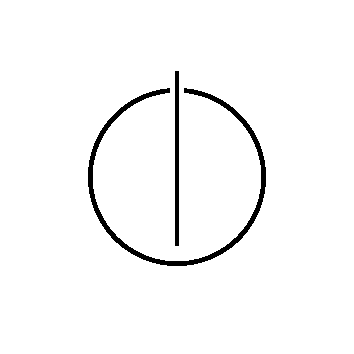
\includegraphics[width=4cm]{styles/informat.png}
  \end{figure}
  
  \end{center}
%	\clearemptydoublepage
%	
%	% The titlepage for the CAMP report document.
% Included by MAIN.TEX


%--------------------------------------------------
% The title page
%--------------------------------------------------

% correct BCOR - undo at the end !!!
\def\bcorcor{0.15cm}
\addtolength{\hoffset}{\bcorcor}

\thispagestyle{empty}

 \vspace{10mm}
\begin{center}
	       \oTUM{4cm}
	   
	   \vspace{5mm}     
	   \huge FAKULT{\"A}T F{\"U}R INFORMATIK\\ 
	   \vspace{0.5cm}
	 \large DER TECHNISCHEN UNIVERSIT{\"A}T M{\"U}NCHEN\\
        
	\end{center}
		

\vspace{10mm}
\begin{center}

   {\Large \doctype}

  \vspace{10mm}
  
  {\LARGE \title}\\
  
  
  \vspace{10mm}
  
  
  {\LARGE  \titleGer}\\
  
  
  \vspace{10mm}

    %\hfill
    \begin{tabular}{ll}
	   \Large Author:     & \Large \author \\[2mm]
	   \Large Supervisor:    & \Large Prof. Dr. Claudia Eckert\\[2mm]				
	   \Large Advisor:	& \Large M.Sc. Paul-Ioan Muntean\\[2mm]
	   \Large Date:       & \Large November 15, 2015
	 \end{tabular}
	 
	 \vspace{5mm}
	 
	 \begin{figure}[h!]
  \centering
   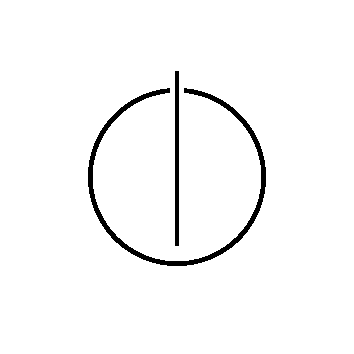
\includegraphics[width=4cm]{styles/informat.png}
  \end{figure}
   

\end{center}

% undo BCOR correction
\addtolength{\hoffset}{\bcorcor}
	
	
%	\input{components/cover_maschmeyer}
	\clearemptydoublepage
	
	% The titlepage for the CAMP report document.
% Included by MAIN.TEX


%--------------------------------------------------
% The title page
%--------------------------------------------------

% correct BCOR - undo at the end !!!
\def\bcorcor{0.15cm}
\addtolength{\hoffset}{\bcorcor}

\thispagestyle{empty}

 \vspace{10mm}
\begin{center}
	       \oTUM{4cm}
	   
	   \vspace{5mm}     
	   \huge FAKULT{\"A}T F{\"U}R INFORMATIK\\ 
	   \vspace{0.5cm}
	 \large DER TECHNISCHEN UNIVERSIT{\"A}T M{\"U}NCHEN\\
        
	\end{center}
		

\vspace{10mm}
\begin{center}

   {\Large \doctype}

  \vspace{10mm}
  
  {\LARGE \title}\\
  
  
  \vspace{10mm}
  
  
  {\LARGE  \titleGer}\\
  
  
  \vspace{10mm}

    %\hfill
    \begin{tabular}{ll}
	   \Large Author:     & \Large \author \\[2mm]
	   \Large Supervisor:    & \Large Prof. Dr. Claudia Eckert\\[2mm]				
	   \Large Advisor:	& \Large M.Sc. Paul-Ioan Muntean\\[2mm]
	   \Large Date:       & \Large November 15, 2015
	 \end{tabular}
	 
	 \vspace{5mm}
	 
	 \begin{figure}[h!]
  \centering
   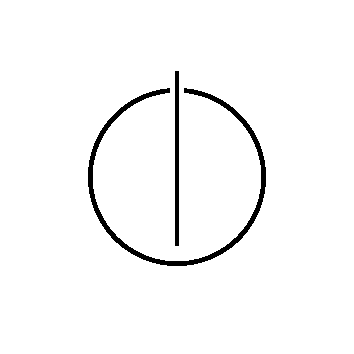
\includegraphics[width=4cm]{styles/informat.png}
  \end{figure}
   

\end{center}

% undo BCOR correction
\addtolength{\hoffset}{\bcorcor}
	
	
	\clearemptydoublepage


\thispagestyle{empty}
\selectlanguage{german}
	\vspace*{0.8\textheight}
	\noindent
	Ich versichere, dass ich diese Diplomarbeit selbst{\"a}ndig verfasst und nur 
	die angegebenen \\Quellen und Hilfsmittel verwendet habe.
	
	\vspace{15mm}
	\noindent
	M{\"u}nchen, den \today \hspace{5cm} \author
\selectlanguage{english}
\newpage
	
	\clearemptydoublepage
\phantomsection
\addcontentsline{toc}{chapter}{Acknowledgements}	


%\chapter*{Acknowledgements}

\vspace*{2cm}

\begin{center}
{\Large \bf Acknowledgments}
\end{center}

\vspace{1cm}




I would like to express my deepest appreciation to all those who provided me the possibility to complete this thesis. A special gratitude and thanks I give to my supervisor Prof. Dr. Claudia Eckert and my advisor, MSc. Paul Muntean, whose guidance, stimulating suggestions and encouragement, helped me in all the time of research and writing of this thesis. Without their cooperation in the last 6 months, this thesis could not be done smoothly.

Last but not the least, I wish to thank my family for their support and encouragement throughout my Master study.
	
	% Abstract for the TUM report document
% Included by MAIN.TEX


\clearemptydoublepage
\phantomsection
\addcontentsline{toc}{chapter}{Abstract}	





\vspace*{2cm}
\begin{center}
{\Large \bf Abstract}
\end{center}
\vspace{1cm}

Information flow vulnerabilities detection with static code analysis techniques is challenging because code
is usually not available during the software design phase and
previous knowledge about what should be annotated and tracked
is needed. To detect information flow errors in UML state
charts and C code are not easy task as they can cause data leakages or unexpected program behavior. In this research it is proposed that textual annotations used to
introduce information flow constraints in UML state charts and code which are afterwards automatically loaded by information flow checkers that check if imposed constraints hold or not. The experimental results on selected sample scenarios shows that this approach
is effective and can be further applied to other types of UML
models and programming languages as well, in order to detect
different types of vulnerabilities.

The contributions of this thesis is the development of a system for semi-automated detection of sanitization, authentication and declassification errors in UML state charts. A light-weight security annotation language is used in order to define information flow constraints regarding authentication, declassification and santization function errors  in UML state charts and source code.  Annotation language editor is designed as eclipse
plug-ins which is used to edit UML state charts and
source code files. Developed Source code generator as eclipse plug-in which is used to generate C code with header files from UML State chart. And finally experimented automatic loading and usage of textual annotations inside 3 new checkers.

	\tableofcontents
  
  \clearemptydoublepage

\phantomsection
\addcontentsline{toc}{chapter}{Outline of the Thesis}

\begin{center}
	\huge{Outline of the Thesis}
\end{center}


%--------------------------------------------------------------------
%\section*{Part I: Introduction and Theory}

\noindent {\scshape Chapter 1: Introduction}  \vspace{1mm}

\noindent  This chapter presents an overview of the thesis and it's purposes. 

\noindent {\scshape Chapter 2: Background}  \vspace{1mm}

\noindent  This chapter describes the background informations and the essential theories needed for our research. Authentication, declassification and sanitization functionalities are also presented with example in this chapter. Scientific fundamentals 

%--------------------------------------------------------------------
%\section*{Part II: Implementation and Analysis}

\noindent {\scshape Chapter 3: Challenges and Annotation Language Extension}  \vspace{1mm}

\noindent  This chapter presents the challenges and annotation language extension for the system. Annotation language extension process, what technology and tools are used to develop and how it works are also presented inside this chapter.

\noindent {\scshape Chapter 4: Implementation}  \vspace{1mm}

\noindent  This chapter presents the implementation of the system. Implementation mechanism, technology and tools which have been used to develop the system are also presented inside this chapter.

\noindent {\scshape Chapter 5: Experiments}  \vspace{1mm}

\noindent  This chapter presents the different application areas of the system. Inside this chapter the system is checked for three real-life scenarios and presented the outcome of the system. 

\noindent {\scshape Chapter 6: Related Work}  \vspace{1mm}

\noindent  This chapter presents some of the related work of this research. Some of the related tools that have been already developed and comparison with them are also presented inside this chapter.


%--------------------------------------------------------------------
%\section*{Part III: Conclusion and Future Works}

\noindent {\scshape Chapter 7: Limitations, Conclusion and Future Work}  \vspace{1mm}

\noindent  This chapter presents the limitations of this research, conclusion of the whole research along with future work intentions.

	\mainmatter
	
	
		% ---------------------------------------------------------------------------
		%
		%Introduction and Background Theory
		%
		% ---------------------------------------------------------------------------
		\part[Introduction and Theory]{Introduction and Theory}
		\label{part:introAndBackgroundTheory}
		\chapter{Introduction}
\label{chapter:Introduction}

The detection of information flow vulnerabilities uses dynamic analysis techniques , static analysis techniques and hybrid techniques which combine static and dynamic approaches. The static techniques need to know when to use  sanitization , declassification and authentication functions.
A solution for tagging sanitization, declassification and authentication in source code is based on libraries which contain all needed annotations attached to function declarations. This approach plays an important role mainly for static analysis bug detection techniques where the information available during program run-time is not available nor the interaction with the environment can be fully simulated.
Extended Static Checking (ESC) is a promising research area which tries to cope with the shortage of not having the program run-time information. During extended static analysis additional information is provided to the static analysis process. This information can be used to define trust boundaries and tag variables. Textual annotations are usually manually added by the user in source code. At the same time annotations can be automatically generated and inserted into source code . ESC can be used to eliminate bugs in a late stage of the software project when code development is finished. Tagging and checking for information exposure bugs during the design phase would eliminate the potential of implementing software bugs which can only be removed very costly after wards. Thus security concerns should be enforced into source code right after the conceptual phase of the project.
The paper presents five challenges concerning ESC. The last challenge reports of the annotation as being a very time consuming burden and is therefore disliked by some programming
teams. The authors argue about the fact that annotations can cover design decisions and enhance the quality of source code. We argue that annotations are necessary in order to do ESC and the user needs a kind of assistance tool that helps selecting the suited annotation based on the current context. Thus the annotation burden needed for learning and applying the language should be reduced. At the same time adding annotations to reusable code libraries reduces even more the annotation burden since libraries can be reused, shared and changed by software development
teams.\\

Information flow errors in UML models
and code are introduced by software designers or programmers
who are sometimes blind with respect to the fact that they
are trained to focus point-wise (one code line and one data flow
at a time). This is why it is important to develop techniques
and tools which can detect this type of errors before they
materialize in production code.Information flow vulnerabilities are hard to detect because static code analysis techniques need previous knowledge about what should be considered a security issue. Code annotations which are added mainly during software development [6] can be used to provide additional knowledge regarding security
issues. On the other hand code annotations can increase the
number of source code lines by 10% [27]. In order to detect
information flow vulnerabilities software artifacts have to be
annotated with annotations attached to public data, private data and to system trust boundaries. Next, annotated artifacts have
to be made tractable by tools which can use the annotations
and check if information flow constraints hold or not based on
information propagation techniques.\\

The detection of information flow vulnerabilities in code
and UML state charts is not well addressed and is particularly
challenging. Foremost, there is no common annotation language for annotating UML state charts and source code with
information flow security constraints such that errors can be
detected also when code is not available. Second, there are
no automated checking tools which can reuse the annotated
constraints in early stages of software development to check
for information flow errors. We think that it is important to
specify security constraints as early as possible in the software
development process in order to avoid later costly repairs or
exploitable vulnerabilities.
 
\section{Latex Introduction}
There is no need for a latex introduction since there is plenty of literature out there.
 



		
		
		%
		%% ---------------------------------------------------------------------------
		%%
		%% Fully Automated Calibration for Ultrasound
		%%
		%%% ---------------------------------------------------------------------------
		\part[The 2nd Part]{The Second Part}
		\label{part:secondP}
		
		
		% ---------------------------------------------------------------------------
		%
		% Appendix
		%
		% ---------------------------------------------------------------------------
		
		\part*{Appendix}
		\addcontentsline{toc}{part}{Appendix}
		
		\appendix %---------------------------------------
		
		\chapter{Appendix}
\section{Appendix A: Source Code Editor with Annotation Language}
\lstinputlisting[numbers=left,firstnumber=1,firstline=1]{sourceCode/MyDsl.xtext}

\section{Appendix B: C Code Generator}	

	\lstinputlisting[numbers=left,firstnumber=1,firstline=1]{sourceCode/Naming.xtend}
	
	\lstinputlisting[numbers=left,firstnumber=1,firstline=1]{sourceCode/Types.xtend}
	
\section{Appendix C: Three Checkers in Static Analysis Engine}

\section{Appendix D: Sequence Diagram Generator}

		
	


  \clearemptydoublepage
  
	\bibliography{bibliography/literature}
	
 
\end{document}

